%\vspace{-1ex}
%%%%%%%%%%%%%%%%%%% Section 8 %%%%%%%%%%%%%%%%%%%%%%%
\section {Experimental Results}
\label{sec-exp}

Using real-world and synthetic dataset, we experimentally verify the efficiency and effectiveness of our backbone-based techniques. %Algorithm \approxabd and \heuabd.

\stitle{Datasets}. We used four real-world graphs, including (1) \textbf{{\em Yelp}} \footnote{\scriptsize\url{ http://www.yelp.com/dataset_challenge}}, a restaurant review graph that contains 244,012 edges and 25,881 nodes. Each node includes 10 attributes that are scores of the top-10 high frequency review keywords and the edge reflects that two restaurants are mutually to be one of the 10 nearest neighbors; (2) \textbf{{\em Weibo}} \footnote{\scriptsize\url{https://aminer.org/data-sna}}, a social network graph that contains 732,143 edges and 161,237 nodes. Each node represents a user that includes 6 attributes and the edge reflects "following" relationship; (3) \textbf{{\em Citation}}  \footnote{\scriptsize\url{https://aminer.org/citation}}, an academic network that contains 2,044,459 edges and 1,544,605 nodes. Each node represents a paper that includes 6 attributes and the edge reflects citation relationship; (4) \textbf{{\em YouTube}}  \footnote{\scriptsize\url{http://netsg.cs.sfu.ca/youtubedata/}}, a video recommendation network graph that contains 2,509,862 edges and 129,907 nodes. Each node represents a video that includes 8 attributes and the edge connects one video and the other related videos recommended by YouTube; (5)\warn{research more benchmark datasets if possible}

We also developed a synthetic graph generator
based on GTgraph\footnote{\scriptsize\url{http://www.cse.psu.edu/~kxm85/software/GTgraph/}}
controlled by node distribution models,
graph size as edge number $|E|$ ,
density $d$ and attribute numbers $|\A|$. We applied Magfit \footnote{\scriptsize\url{http://snap.stanford.edu/snap/index.html}} to generate  attribute values.

\vspace{.5ex}
For all datasets, we
sample $V_I$ by issuing
entity search queries with terms
of interests, such as conference topics for \cita,
and the range of hitting volume for \youtube.

\stitle{Algorithms}. We implemented the following \eat{in Java} algorithms. 
(1) Algorithms \approxabd, \heuabd and \heuabd + learning. Here 
the algorithm \heuabd + learning performs a {\em once-for-all} \EM-based
learning process and learns the generation model; and 
\heuabd refers to the algorithm that starts with a learned affinity matrix, 
and grows backbones by iteratively selecting attributes that can minimize an expected edge cost for the backbone.  
%\reviseS{Here \heuabd refers to the algorithm that starts with a learned affinity matrix. \heuabd only grows backbone by iteratively selecting attributes that can minimize an expected edge cost for the backbone.  Given any graph, the affinity matrix learning is invoked only once for one graph.}  ;
(2) \naive, a variant of \approxabd that
transforms $G$ to a multigraph $\G$ directly, and
performs clustering scheme to compute prize-collecting Steiner tree.
(3) \cesna~\cite{yang2013community}, a
state-of-the-art algorithm that returns
communities as node sets with associated attributes.
(4) \kcore~\cite{khaouid2015k},
which detects connected subgraphs.
(5) \ks, a keyword search algorithm 
that implements 
state-of-the-art algorithm~\cite{gubichev2012fast} 
to induce minimum Steiner trees over $V_I$ 
as backbones. 
\vspace{.5ex}
\warn{For online setting comparison, we add several other algorithms.}

(6)\warn{batch-mode window size online algorithm;}

(7)\warn{online approxABD algorithm;}

(8)\warn{online fastABD algorithm.}

\vspace{.5ex}
For (1) and (2), the costs $c(.)$ in the experiment are calculated by taking dissimilarity measures, We 
define the common attribute set between $v_i$ and $v_j$ as ${\A_{ij} = \A(v_i)\cap\A(v_j)}$. Then, ${c(v_i,v_j) = \frac{\sum_{A \in \A_{ij}}d_{ij}(A)}{|\A_{ij}|}}$, where ${\A_{ij} \neq \emptyset}$. $d_{ij}(A)$ stands for the distance between the common attribute values of $A$ of node $v_i$ and $v_j$. For (3), we retain the settings described in the paper of \cesna and consider all returned vertices as one big community. For (4), \kcore returns the coreness of each vertex in $G$. We sort the value of coreness from the largest to the smallest and only consider nodes with top-$k$ coreness values to form an important community since the larger coreness value represents higher degrees and requires more attention. In the experiment, we set $k$ as 20.

\begin{figure}[tb!]
\centering
	\begin{center}
	%%%%%%%%%%%%%%%%%%%%%%%%%%%%%%%%%%
		\subfigure[Efficiency]{\label{fig-eff-real}
			{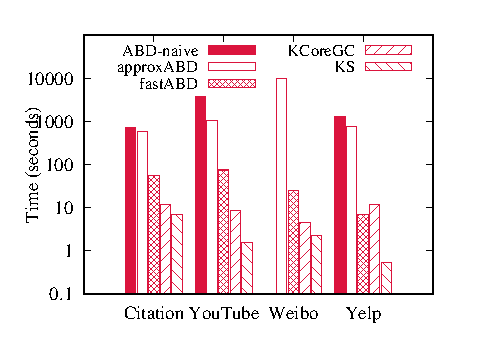
\includegraphics[width=4cm,height=3cm]{exp/Time_real_effeciency_v3}}}
			%%%%%%%%%%%%%%%%%%%%%%%%%%%%%%%%%
		\hfill\subfigure[Effectiveness: node loss]{\label{fig-effe-real}
			{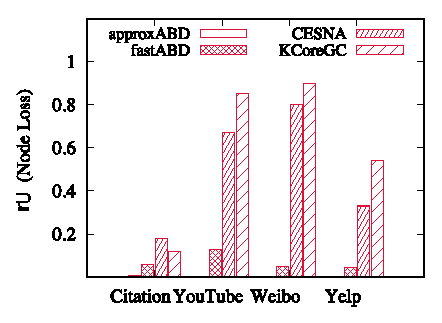
\includegraphics[width=4cm,height=3cm]{exp/Time_real_effectiveness_v3}}}
			%%%%%%%%%%%%%%%%%%%%%%%%%%%%%%%%%
	\end{center}
\vspace{-2ex}
\caption{Performance on real-world graphs}
\label{fig:real1}
%\vspace{-4ex}
\end{figure}

\stitle{Metrics}. For \heuabd, we report
the once-for-all learning time cost, and the
inference time that constructs backbones from the model $\M$.
We use two loss metrics applicable to
all the algorithms
for a fair comparison.
Denote the subgraph returned by an
algorithm as $G_T$,
(1) the node loss ratio $r_u$ = 1- $\frac{|V_T\cap V_I|}{|V_I|}$,
\ie the fraction of $V_I$
not covered by $G_T$, and
(2) the interestingness loss ratio $r_I$ = $\frac{\sum_{v\in V_I\setminus V_T} I(v)}{\sum_{v\in V_I}I(v)}$, where $V_T$ is the node set of $G_T$.
\eat {We also compare the cost $C(T)$
for \abd algorithms.}
For all metrics, the smaller, the better the backbones are.
(3) \warn{a potential new metric based on benchmark dataset needs to be added.}


\vspace{.5ex}
We ran all our experiments on a Linux machine powered by an
Intel $2.4$ GHz CPU with $128$ GB of memory.
We ran each test $5$ times, and report the averaged results. Our source code and test cases are available online.\footnote{\scriptsize\url{https://github.com/wsu-db/Attribute-Driven-Backbone-}}

\begin{figure}[tb!]
	\addtolength{\subfigcapskip}{0in}
	\begin{center}
	%%%%%%%%%%%%%%%%%%%%%%%%%%%%%%%%%%
		\subfigure[Varying $|E|$]{\label{fig-eff-g}
			{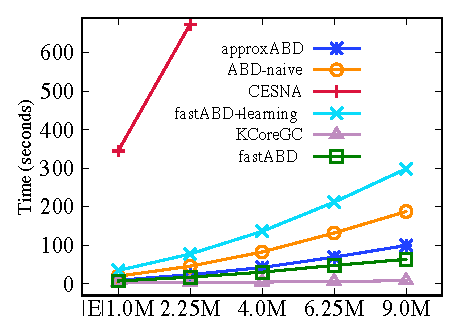
\includegraphics[width=4cm,height=3cm]{exp/Time_varying_E__efficiency}}}
			%%%%%%%%%%%%%%%%%%%%%%%%%%%%%%%%%
		\hfill\subfigure[Varying $d$]{\label{fig-eff-d}
			{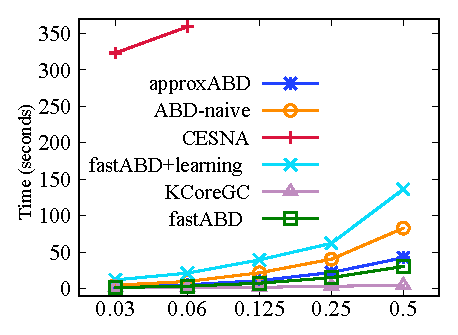
\includegraphics[width=4cm,height=3cm]{exp/Time_varying_D__efficiency}}}
			%%%%%%%%%%%%%%%%%%%%%%%%%%%%%%%%%
        \vskip\baselineskip
		\subfigure[Varying Network Model]{\label{fig-eff-Dis}
			{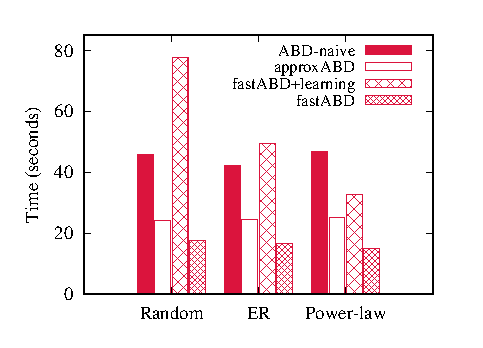
\includegraphics[width=4cm,height=3cm]{exp/Time_varying_Distribution_effeciency_v3}}}		
			%%%%%%%%%%%%%%%%%%%%%%%%%%%%%%%%%
		\hfill\subfigure[Varying $|\A|$]{\label{fig-eff-A}
			{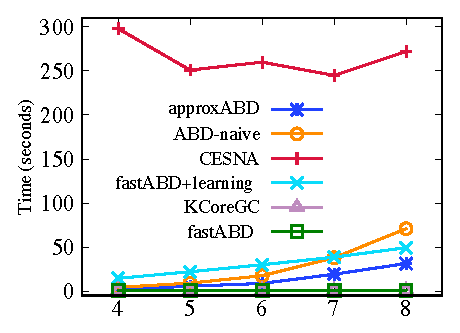
\includegraphics[width=4cm,height=3cm]{exp/Time_varying_A__efficiency.eps}}}
	\end{center}
	\vspace{-2ex}
	\caption{Efficiency: synthetic graphs}\label{fig-efficiency}
%	\vspace{-4ex}
\end{figure}

\vspace{.5ex}
We next present the details of our findings.

\stitle{Exp-1: Efficiency}.
We first report the efficiency of \approxabd, \heuabd, and \naive, compared with \cesna, \ks, and \kcore on real-world datasets, as shown in Fig.\ref{fig-eff-real}.
We sample interested nodes for each dataset.
 \cesna does not run to completion after $3$ hours for all
 datesets; same for \naive over \weibo.
 \eat{heuabd is more feasible over larger networks
 with performance comparable to \kcore and \ks without
 attribute enumeration.}  \heuabd is quite feasible over larger networks. For 
 example, (1) \heuabd takes up to 75 seconds over all the cases; (2) it improves \approxabd and \naive
 by 14 and 49 times respectively on Youtube; (3) it achieves 
 comparable performance with \kcore and \ks without
 attribute enumeration. 
On average, \approxabd outperforms
 \naive by 2.1 times due to more efficient clustering and 
 affinity attribute selection process. \kcore and \ks take less time,
 yet only return structures without attributes. 

%\blue{Then, we report the efficiency performance of $5$ methods on the synthetic dataset.}

\vspace{.5ex}
We next report the impact of several factors to the efficiency
of the algorithms, over larger synthetic graphs under network models.

\etitle{Varying graph size}. Fixing attribute size $|\A|$ = 2, density $d$ = 0.5 ($d=\frac{2|E|}{|V||V-1|}$), interested node set size $|V_I|$=250, we varied $|E|$ from $1$ million to $9$ million under the Random, Erdos-Renyi and Power-Law
distribution models. As shown in Fig. \ref{fig-eff-g},
algorithms \approxabd and \heuabd%, and \naive 
are quite feasible over large networks.
Specifically, \approxabd and \heuabd improves \naive
by 1.95 and 2.72 times, respectively. The once-for-all
learning cost of \heuabd takes up to 300 seconds over
a network with $9$ million edges \eat{and 18 million attributes}.

\etitle{Varying $d$}. Fixing $|V|$, $|\A|$, $|V_I|$
as 4000, 2 and 250, respectively, we varied the density
of $G$ from 0.03 to 0.5. As shown in Fig. \ref{fig-eff-d},
all algorithms take longer time over denser networks as more affinitive edges
need to be inspected.

\etitle{Varying Distribution and $|\A|$}. We are also interested in
the efficiency over different network models. As shown
in Fig. \ref{fig-eff-Dis}, the performance of
our algorithms over synthetic graphs are consistent with their real-world counterparts. 
The total cost of \heuabd
including learning cost is comparable with
the cost of \approxabd. Its inference cost
only takes up to $39\%$ of the cost of \naive.
%%%%%%%%%%%%%%%%%%%%%%%%%%%%%%%%
Fig.~\ref{fig-eff-A} verifies that \approxabd and \naive
take more time when $|\A|$ is larger; while for all cases,
they take up to $70$ seconds to identify backbones from networks with $8$ attributes
(where $|E|$, $d$ and $|V_I|$ are set as
62500, 0.008 and 250, respectively).

%We provide 3 distributions As shown in Fig. \ref{fig-efficiency} (d), \warn{tbf.}.

\begin{figure}[tb!]
    \addtolength{\subfigcapskip}{0in}
    \begin{center}
    \subfigure[Interestingness loss vs density]{\label{fig-effe-ri-d}
		{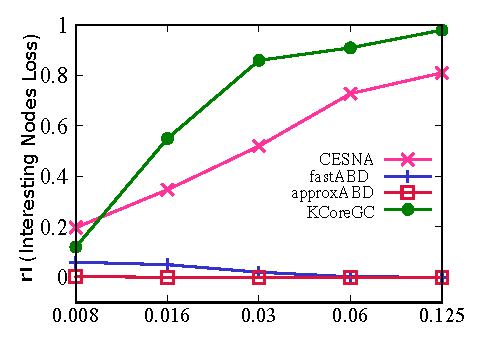
\includegraphics[width=4cm,height=3cm]{exp/piFEffect_VaryingD.eps}}}		
		%%%%%%%%%%%%%%%%%%%%%%%%%%%%%%%%%
    \hfill\subfigure[Node loss vs. density]{\label{fig-effe-ru-d}
		{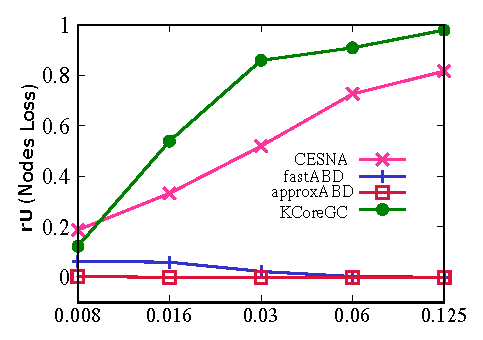
\includegraphics[width=4cm,height=3cm]{exp/ratioEffect_VaryingD.eps}}}
		%%%%%%%%%%%%%%%%%%%%%%%%%
		 \subfigure[Interestingness loss vs. $|\A|$]{\label{fig-effe-ri-A}
        {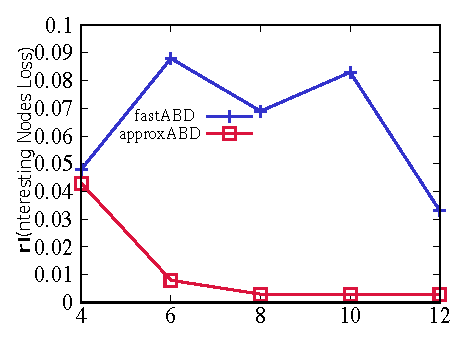
\includegraphics[width=4cm,height=3cm]{exp/piFEffect_VaryingA.eps}}}
        %%%%%%%%%%%%%%%%%%%%%%%%%%%%%%%%%
    \hfill\subfigure[Node loss vs. $|\A|$]{\label{fig-effe-ru-A}
        {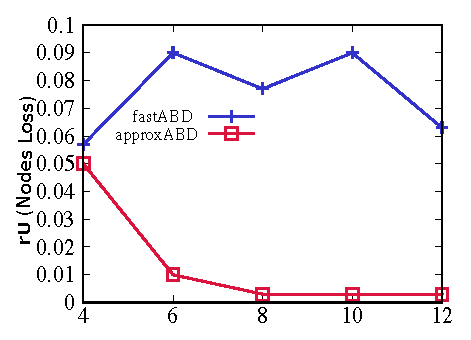
\includegraphics[width=4cm,height=3cm]{exp/ratioEffect_VaryingA.eps}}}
	\end{center}
	\vspace{-3ex}
	\caption{Effectiveness: synthetic graphs }\label{fig-effectiveness1}
%	\vspace{-4ex}
\end{figure}

\vspace{.5ex}
\stitle{Exp-2: Effectiveness}.
We report the node loss $r_u$ of the  algorithms
in Fig.~\ref{fig-effe-real}. To ensure that all the algorithms 
run to completion, we randomly sampled real-world graphs and created 
connected subgraphs with $|E|$=62,500. 
As \ks always cover
all the interested nodes, and
\naive has the same result as
\approxabd, their results are not shown. 
\approxabd has the smallest
coverage loss, while \cesna and \kcore
easily lose more than $60\%$ of the
interested nodes over denser graphs.
This is because both algorithms
tend to return results that are "skewed"
to high-degree nodes, leading to
a larger missing rate
for random interested nodes.

\vspace{.5ex}
We next evaluate the impact of density $d$ and
$|\A|$. Fixing $|V|$=4000, $|\A|$=2, $|V_I|$=250,
we varied $d$ from 0.008 to 0.125.
Fig.~\ref{fig-effe-ri-d} and Fig.~\ref{fig-effe-ru-d}
show that it is
more likely for \approxabd and \heuabd to find better
backbones and reduce both node and interestingness loss
in denser graphs.
On the other hand, both \cesna and \kcore
have higher chance to lose interested nodes,
due to the distraction of high degree nodes
and dense areas. This is consistent with
the result in Fig.~\ref{fig-effe-real}.

\vspace{.5ex}
Fixing $|E|$= 62500, $d$= 0.008, $|V_I|$=300,
we varied $|\A|$ from 4 to 12. Figs. \ref{fig-effe-ri-A} and  \ref{fig-effe-ru-A} show that more attribute values
help \approxabd to find better backbones.The result constantly gets improved, ensured
by its approximation scheme. \heuabd is less
sensitive to $\A$. We also found that
it infers better backbones if more attributes
are inferred (by setting larger $k$; not shown).

\stitle{Exp-3: Case analysis}.
Fig.~\ref{fig-case-1} and Fig.~\ref{fig-case-2}
illustrate real-world backbones
from \approxabd over \weibo and
\cita, respectively.

\stab
(1) The social backbone on \weibo
connects users having common
topic on ``Langlangconcert''
(interested users; marked in orange)
via close users determined by
various affinitive
attributes indicating same genders, ages, locations
or common topics. We observed that such backbones can provide intuitive 
information that suggest how two entities are connected. For example, user 2 and user 3 both tweet ``Langlangconcert'' with strong correlation to location and 
age range. The backbone can be used to suggest 
potential communities that include a group of %interested users %as many as possible and
users along with new social relationship under various similar 
properties. %This distinguishes our work with existing community detection. 
Community models without affinity attributes and 
assume fixed topology constraints~\cite{zhang2017engagement} can not be applied to characterize 
such structures. 

\stab
(2) The academic backbone on \cita
suggests potential collaborators driven by their
potential co-authorship,
common research topics or
venues (marked by red; Fig.~\ref{fig-case-2}). We found that
\cesna \eat{and \kcore} can only discover
a small fraction induced by
attributed community set
with Author nodes \{1,2,3\},\{4,5,8\} (missing Authors 6 and 7),
and \kcore stops at
k-cores including only
the Author nodes\{1,5,6\} .

\begin{figure}[tb!]
\centering
\centerline{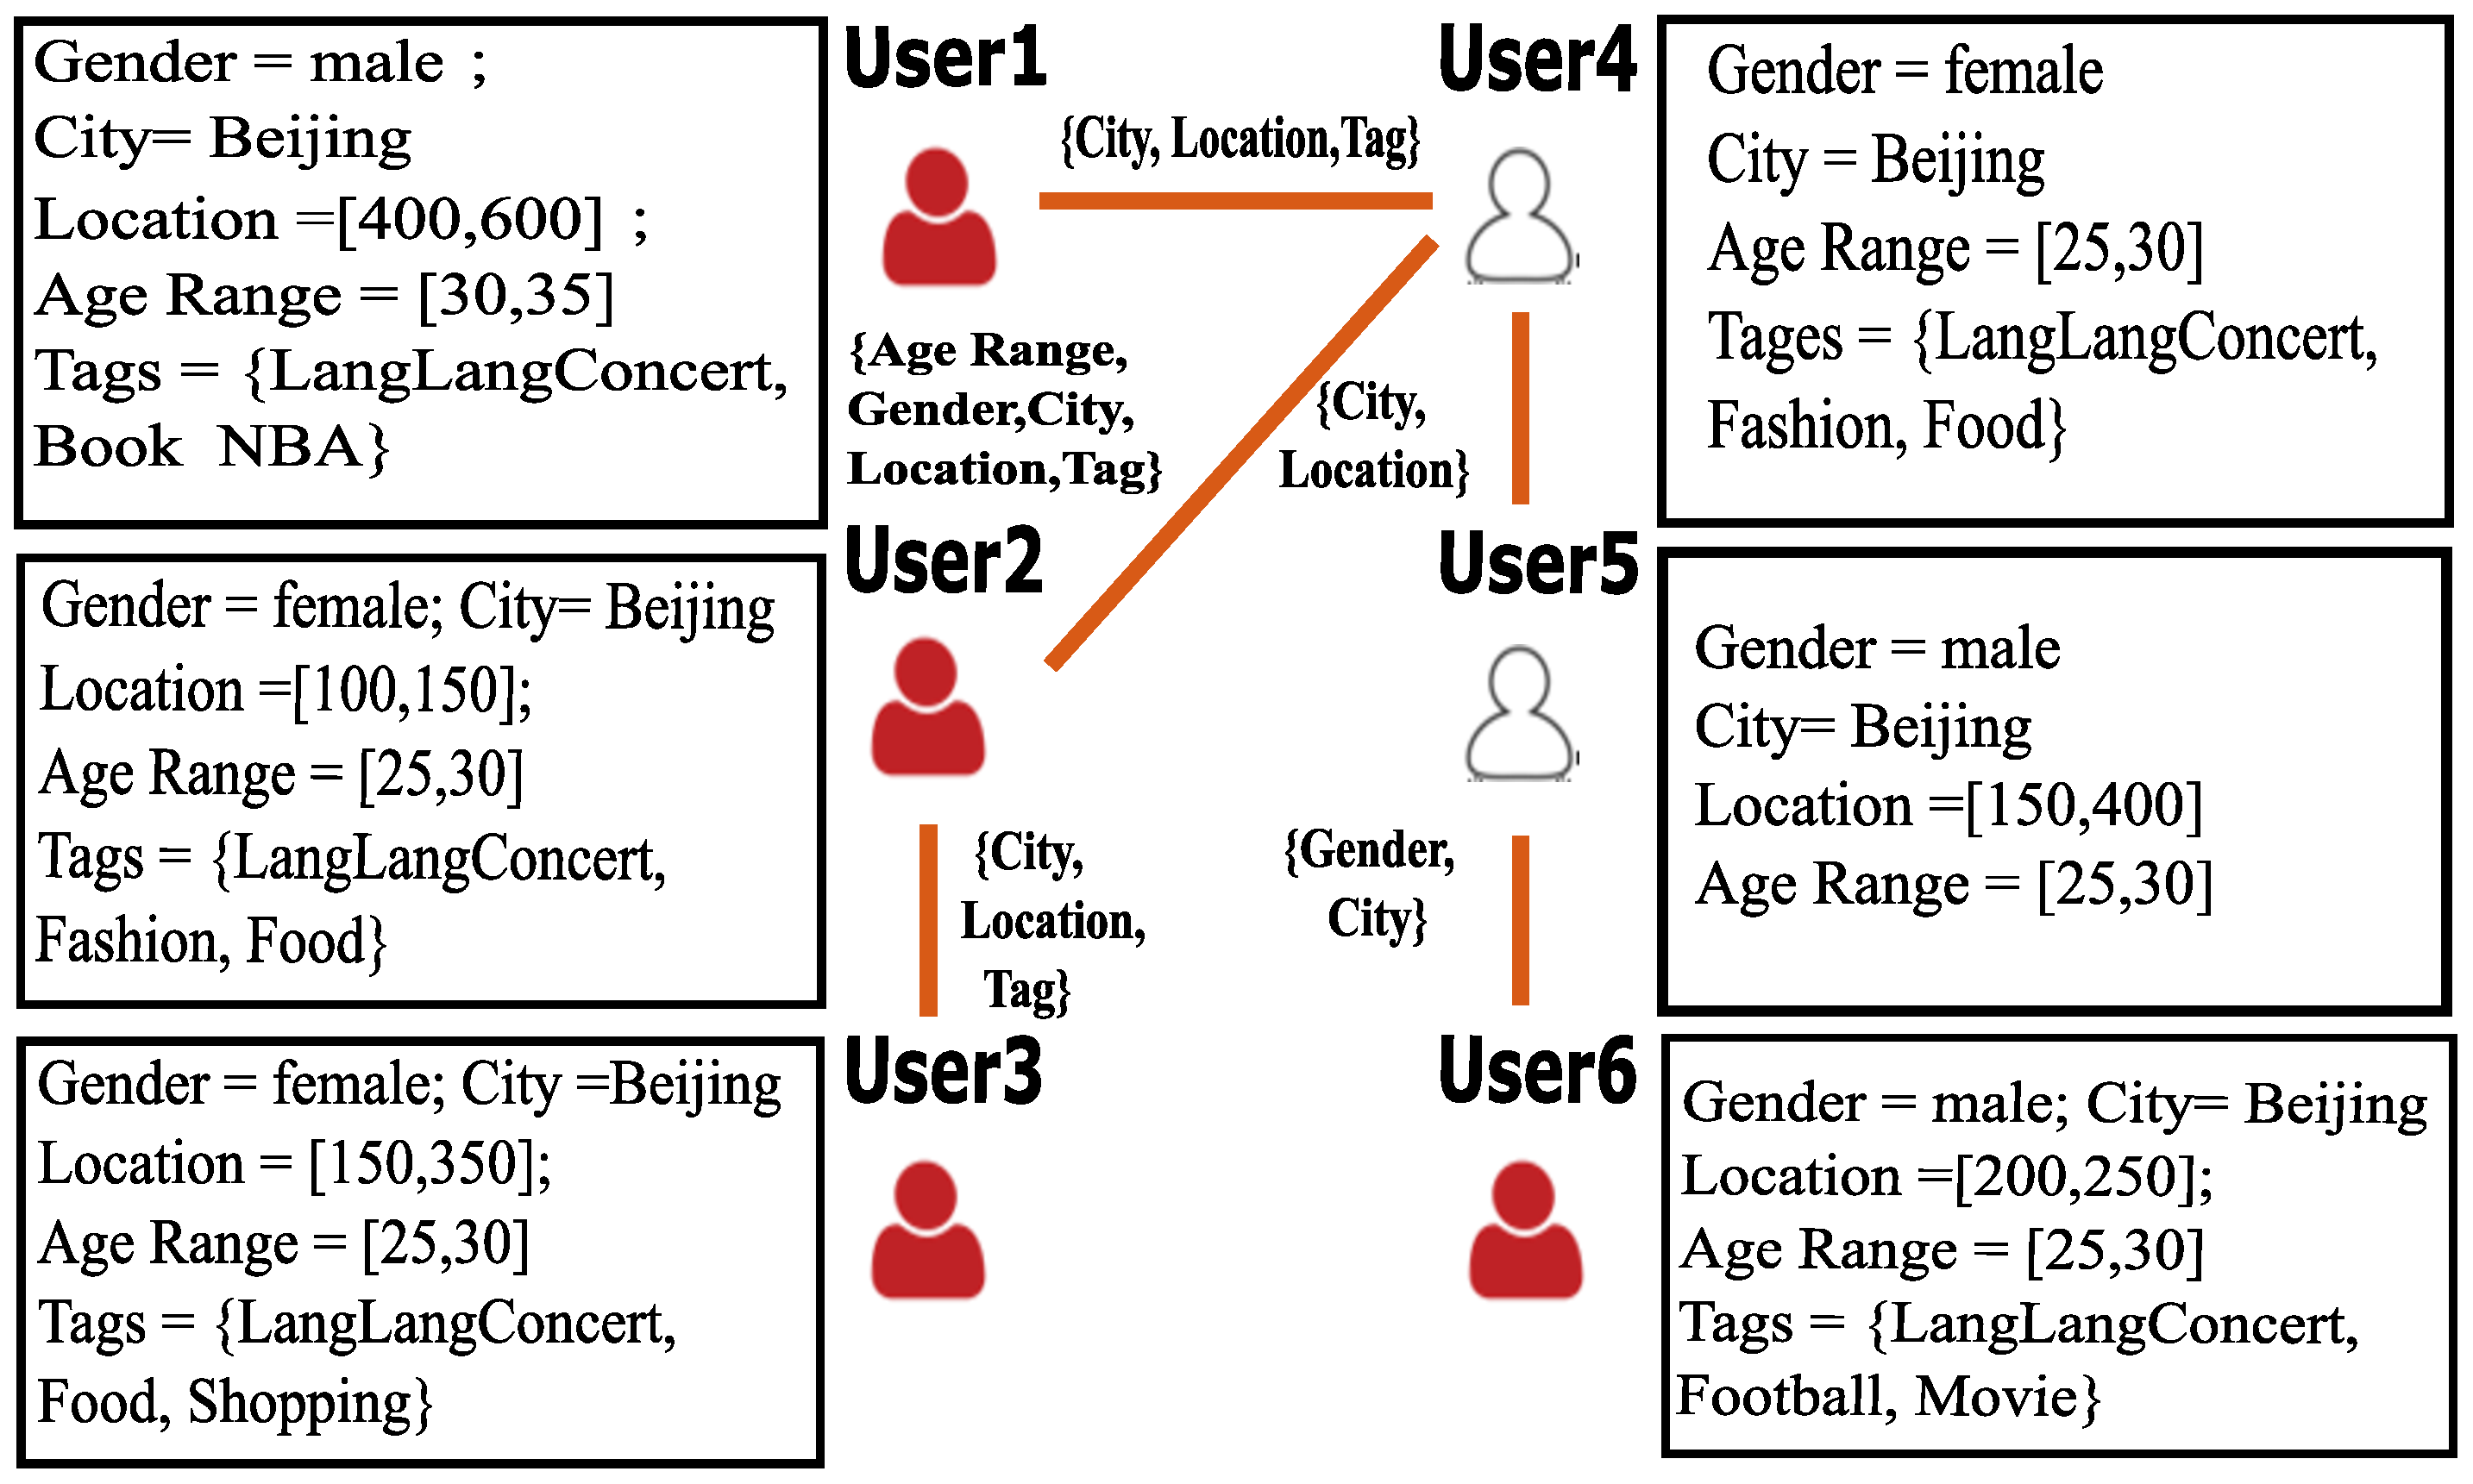
\includegraphics[scale=0.18]{./fig/UseCase1_v3.eps}}%NewMotivationExamplev2
\caption{A social backbone of Weibo users
}
\label{fig-case-1}
%\vspace{-2ex}
\end{figure}

\begin{figure}[tb!]
\centering
\centerline{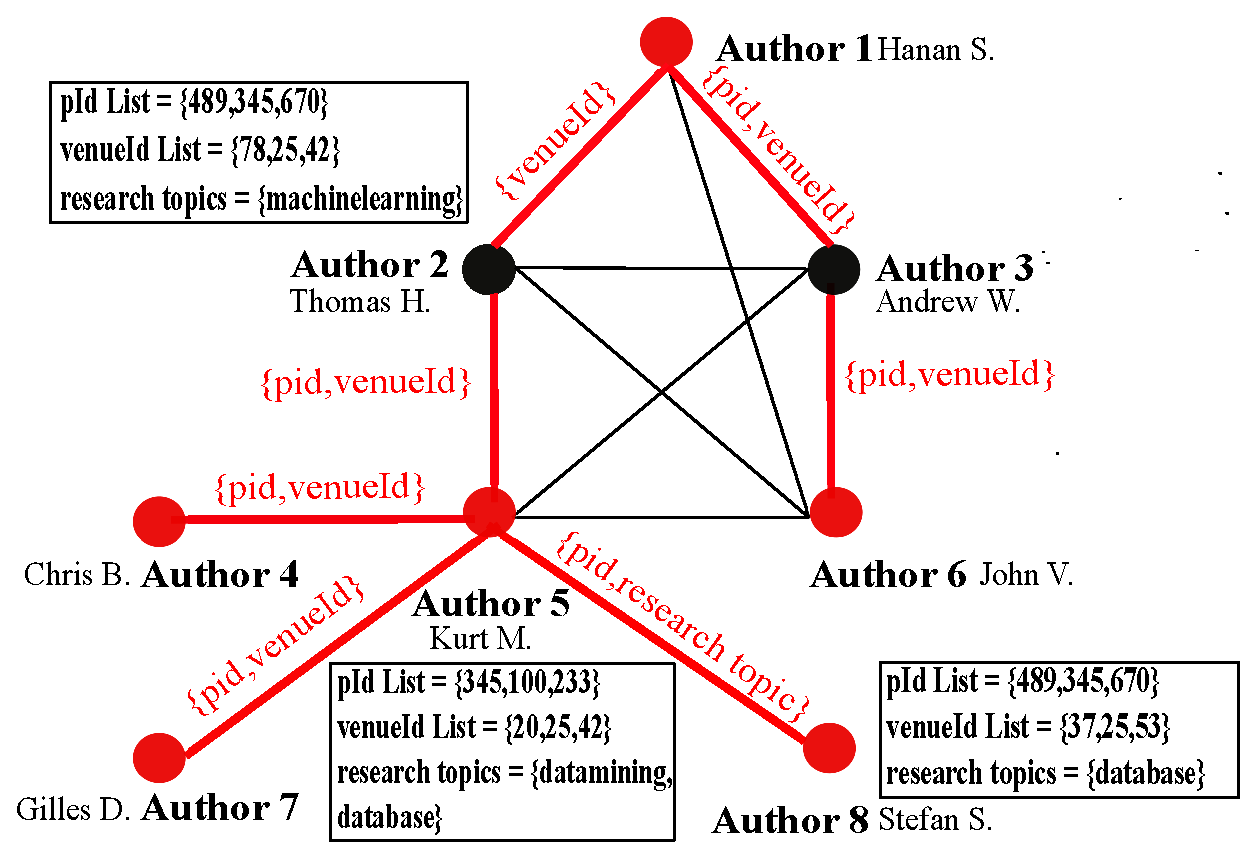
\includegraphics[scale=0.41]{./fig/UseCase2_v3.eps}}%NewMotivationExamplev2
\caption{Academic  Backbone
}
\label{fig-case-2}
%\vspace{-2ex}
\end{figure}

\stitle{Exp-4: Efficiency in online setting}.

\stitle{Exp-5: Effectiveness in online setting}.

\stitle{Exp-6: Case Study in online setting}.